\documentclass{standalone}
\usepackage{tikz}
\usetikzlibrary{shapes.geometric}
\newcommand{\repeater}[3]{%
 \node ({#1}) at ({#2}) {%
  \begin{tikzpicture}%
   \draw [black,thick] (-.25,0) -- (0,0.5) -- (0.25,0) -- (-0.25,0);%
   \draw [black,thick,domain=-45:225] plot ({0.2*cos(\x)}, {0.5+0.2*sin(\x)});%
   \draw [black,thick,domain=-45:225] plot ({0.4*cos(\x)}, {0.5+0.4*sin(\x)});%
   \node (xxx) at (0,-.2) {{#3}};%
  \end{tikzpicture}%
 } %
}

\newcommand{\activerepeater}[3]{%
 \node ({#1}) at ({#2}) {%
  \begin{tikzpicture}%
   \draw [black,thick] (-.25,0) -- (0,0.5) -- (0.25,0) -- (-0.25,0);%
   \draw [red,thick,domain=-45:225] plot ({0.2*cos(\x)}, {0.5+0.2*sin(\x)});%
   \draw [red,thick,domain=-45:225] plot ({0.4*cos(\x)}, {0.5+0.4*sin(\x)});%
   \node (xxx) at (0,-.2) {{#3}};%
  \end{tikzpicture}%
 } %
}


\newcommand{\user}[3]{%
 \node ({#1}) at ({#2}) {%
  \begin{tikzpicture}%
   \draw [black,fill=black] (-.25,0) -- (0,0.5) -- (0.25,0) -- (-0.25,0);%
   \draw [black,fill=black] (0,.5) circle (.2); %
   \node (xxx) [text width=0.6cm, align=center] at (-.35cm,-.4) {{#3}};%
  \end{tikzpicture}%
 } %
}

\newcommand{\activeuser}[3]{%
 \node ({#1}) at ({#2}) {%
  \begin{tikzpicture}%
   \draw [red,fill=red] (-.25,0) -- (0,0.5) -- (0.25,0) -- (-0.25,0);%
   \draw [red,fill=red] (0,.5) circle (.2); %
   \node (xxx) [text width=0.6cm, align=center] at (-.35cm,-.4) {{#3}};%
  \end{tikzpicture}%
 } %
}

\begin{document}
 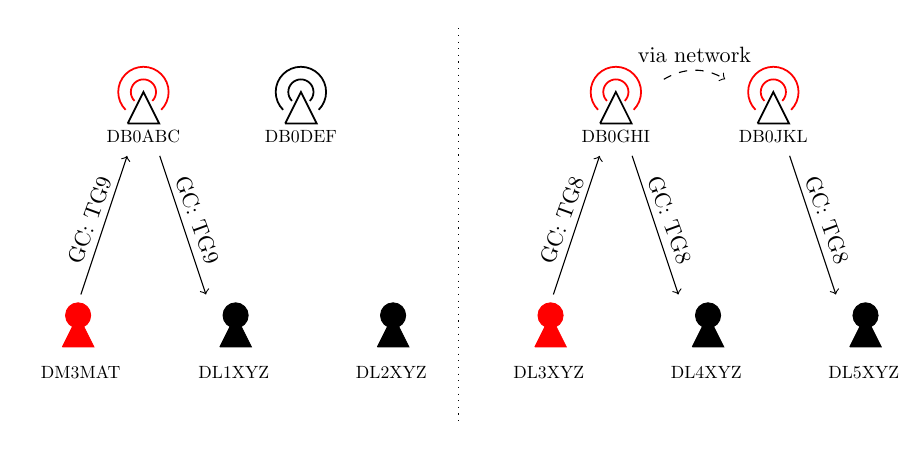
\begin{tikzpicture}[every node/.style={scale=.8}]
  \activeuser{u1}{ 0,0}{DM3MAT};
  \user{u2}{ 2,0}{DL1XYZ};	
  \user{u3}{ 4,0}{DL2XYZ};	
  \draw[dotted] (5,4) -- (5,-1);
  \activeuser{u4}{ 6,0}{DL3XYZ};
  \user{u5}{ 8,0}{DL4XYZ};
  \user{u6}{10,0}{DL5XYZ};
  \activerepeater{R1}{1,3}{DB0ABC};
  \repeater{R2}{3,3}{DB0DEF};
  \activerepeater{R3}{7,3}{DB0GHI};
  \activerepeater{R4}{9,3}{DB0JKL};
  \draw[->] (u1) -- node[above,rotate=70]{GC: TG9} (R1);
  \draw[->] (R1) -- node[above,rotate=-70]{GC: TG9} (u2);
  \draw[->] (u4) -- node[above,rotate=70]{GC: TG8} (R3);
  \draw[->] (R3) -- node[above,rotate=-70]{GC: TG8} (u5);
  \draw[->] (R4) -- node[above,rotate=-70]{GC: TG8} (u6);
  \path[->] (R3) edge[dashed,bend left] node[above]{via network} (R4);
 \end{tikzpicture}
\end{document}
